\documentclass[border = 0.2cm, 12pt]{standalone}
\usepackage{amsmath, amssymb, amsfonts}
\usepackage{color}
\usepackage{tikz, pgfplots}
\pgfplotsset{compat=newest}
\usetikzlibrary{shapes,snakes}
\tikzset{>=latex}
\usetikzlibrary{angles,quotes}
\usepackage{tkz-euclide}

\begin{document}

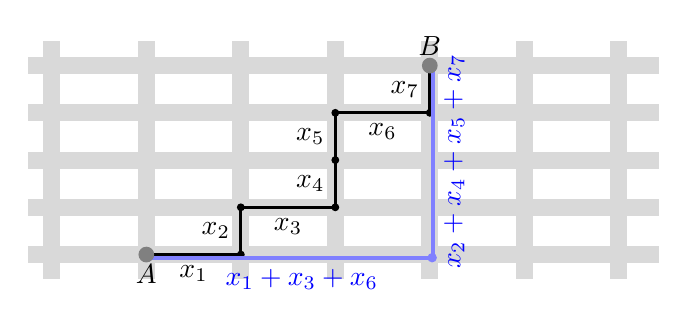
\begin{tikzpicture}[scale=1]

\draw[draw=gray!30, fill=gray!30] (0,0) rectangle ++ (8,0.2);

\draw[draw=gray!30, fill=gray!30] (0,0.6) rectangle ++ (8,0.2);

\draw[draw=gray!30, fill=gray!30] (0,1.2) rectangle ++ (8,0.2);

\draw[draw=gray!30, fill=gray!30] (0,1.8) rectangle ++ (8,0.2);

\draw[draw=gray!30, fill=gray!30] (0,2.4) rectangle ++ (8,0.2);

\draw[draw=gray!30, fill=gray!30] (0.2,-0.2) rectangle ++ (0.2,3);

\draw[draw=gray!30, fill=gray!30] (1.4,-0.2) rectangle ++ (0.2,3);

\draw[draw=gray!30, fill=gray!30] (2.6,-0.2) rectangle ++ (0.2,3);

\draw[draw=gray!30, fill=gray!30] (3.8,-0.2) rectangle ++ (0.2,3);

\draw[draw=gray!30, fill=gray!30] (5,-0.2) rectangle ++ (0.2,3);

\draw[draw=gray!30, fill=gray!30] (6.2,-0.2) rectangle ++ (0.2,3);

\draw[draw=gray!30, fill=gray!30] (7.4,-0.2) rectangle ++ (0.2,3);

\draw[arrows=-, line width=1.2, color=black] (1.5,0.1)--(2.7,0.1) node [midway, below, sloped] (TextNode) {$x_1$};
\fill[black] (2.7,0.1) circle[radius=0.05cm];
\draw[arrows=-, line width=1.2, color=black] (2.7,0.1)--(2.7,0.7) node [midway, left] (TextNode) {$x_2$};
\fill[black] (2.7,0.7) circle[radius=0.05cm];
\draw[arrows=-, line width=1.2, color=black] (2.7,0.7)--(3.9,0.7) node [midway, below, sloped] (TextNode) {$x_3$};
\fill[black] (3.9,0.7) circle[radius=0.05cm];
\draw[arrows=-, line width=1.2, color=black] (3.9,0.7)--(3.9,1.3) node [midway, left] (TextNode) {$x_4$};
\fill[black] (3.9,1.3) circle[radius=0.05cm];
\draw[arrows=-, line width=1.2, color=black] (3.9,1.3)--(3.9,1.9) node [midway, left] (TextNode) {$x_5$};
\fill[black] (3.9,1.9) circle[radius=0.05cm];
\draw[arrows=-, line width=1.2, color=black] (3.9,1.9)--(5.1,1.9) node [midway, below, sloped] (TextNode) {$x_6$};
\fill[black] (5.1,1.9) circle[radius=0.05cm];
\draw[arrows=-, line width=1.2, color=black] (5.1,1.9)--(5.1,2.5) node [midway, left] (TextNode) {$x_7$};

\draw[arrows=-, line width=1.4, color=blue!50] (1.5,0.06)--(5.1,0.06) node [midway, below, sloped] (TextNode) {\color{blue}$\quad x_1+x_3+x_6$};
\fill[blue!50] (5.13,0.06) circle[radius=0.06cm];
\draw[arrows=-, line width=1.4, color=blue!50] (5.14,0.06)--(5.14,2.5) node [midway, below, sloped] (TextNode) {\color{blue}$x_2+x_4+x_5+x_7$};

\fill[gray] (1.5,0.1) circle[radius=0.1cm] node [below] {\color{black}$A$};

\fill[gray] (5.1,2.5) circle[radius=0.1cm] node [above] {\color{black}$B$};

\end{tikzpicture}

\end{document}